% LaTeX Template for Project Report, Version 2.0
% (Abstracted from a Major Project Report at CSED, NIT Calicut but can be
% modified easily to use for other reports also.)
%
% Released under Creative Commons Attribution license (CC-BY)
% Info: http://creativecommons.org/licenses/by/3.0/
%
% Created by: Kartik Singhal
% BTech CSE Batch of 2009-13
% NIT Calicut
% Contact Info: kartiksinghal@gmail.com
%
% It is advisable to learn the basics of LaTeX before using this template.
% A good resource to start with is http://en.wikibooks.org/wiki/LaTeX/
%
% All template fields are marked with a pair of angular brackets e.g. <title here>
% except for the ones defining citation names in ref.tex.
%
% Empty space after chapter/section/subsection titles can be used to insert text.
%
% Just compile this file using pdflatex after making all required changes.

\documentclass[12pt,a4paper]{report}
\usepackage[linesnumbered,lined,boxed,commentsnumbered,ruled]{algorithm2e}
\usepackage[utf8]{inputenc}
\usepackage[english]{babel}
\usepackage{minted}
\usepackage[pdftex]{graphicx} %for embedding images
\usepackage{url} %for proper url entries
\usepackage[bookmarks, colorlinks=false, pdfborder={0 0 0}, pdftitle={<pdf title here>}, pdfauthor={<author's name here>}, pdfsubject={<subject here>}, pdfkeywords={<keywords here>}]{hyperref} %for creating links in the pdf version and other additional pdf attributes, no effect on the printed document
%\usepackage[final]{pdfpages} %for embedding another pdf, remove if not required

\begin{document}
\renewcommand\bibname{References} %Renames "Bibliography" to "References" on ref page

%include other pages
\begin{titlepage}

\begin{center}

% Title
\Large \textbf {KodeFork - An Online Learning Portal}\\[0.5in]

       \small \emph{Report of the project submitted\\
       in partial fulfillment of the requirements\\ for the award of the degree of}
        \vspace{.2in}

       {\bf Bachelor of Technology \\in\\ Computer Science and Engineering}\\[0.5in]


\vspace{.5in}
% Submitted by
\normalsize Submitted by \\\\

  Astik Anand (B130542CS)\\


\vspace{.1in}
Under the guidance of\\
{\textbf{Ms. Anu Mary Chacko}}\\[0.2in]

\vfill

% Bottom of the page

\includegraphics[width=0.18\textwidth]{./nitc-logo}\\[0.1in]
\Large{Department of Computer Science and Engineering}\\
\normalsize
\textsc{National Institute of Technology Calicut}\\
Calicut, Kerala, India -- 673 601 \\
\vspace{0.2cm}
April 2017

\end{center}

\end{titlepage}

\newpage
\thispagestyle{empty}

\begin{center}

\Large{Department of Computer Science and Engineering}\\[0.5cm]

\Large{National Institute of Technology Calicut}\\[2.0cm]

\emph{\LARGE Certificate}\\[2.5cm]
\end{center}
\normalsize This is to certify that this is a bonafide record of the work done by the student whose name is given below during 2016-17 Winter semester in partial fulfilment of the requirements for the award of the degree of Bachelor of Technology in Computer Science and Engineering.\\[1.0cm]

\begin{table}[h]
\centering
\begin{tabular}{lr}
Roll No & Name of Student \\ \\ \hline
\\
B130542CS & Astik Anand \\ 
\end{tabular}
\end{table}

\vfill


% Bottom of the page
\begin{flushright}
\\
Ms. Anu Mary Chacko\\
(Project Guide and Coordinator)\\[1.5cm]
\end{flushright}

\begin{flushleft}
Date: 3 May, 2017
\end{flushleft}

\vspace{2in}
\begin{abstract}

KodeFork Web Portal provides computer science
related courses and concepts. It also provides a community based
question and answering portal. This report focuses on using
Python in Web with it’s most powerful Django framework.It
also make use of MVC(Model View Controller) architecture and
RESTful API. It gives brief introduction about domain of using
Python and Django in web, their benefits and advantages.It also
talks about motivation of doing this project and some high level
problems that will be tackled. Finally it shows the layout and
design of the portal with necessary requirements.

\end{abstract} 

\cleardoublepage
%\pagebreak
\phantomsection
\addcontentsline{toc}{chapter}{Acknowledgements}
\chapter*{Acknowledgments}
\vspace{1.0in}
During  this  year  long  project  several  people  have  provided  many  forms  of  help  and  support.  Firstly, I would  like  to  thank  Ms. Anu Mary Chacko, my project guide and coordinator for  allowing me to  do  this  project  and  for her continuous  guidance  throughout  the  project. Secondly, I would like to thank Dr. Vineeth Paleri, Bharath Narayanan Sir and my panel members for all the help. Finally, I thank our Computer Science and Engineering department and all its faculty members for equipping us with all the necessary tools and knowledge to complete this project.
\\
\\
\\ 
\\
Astik Anand \\
\\
April,2017\\
{National Institute of Technology Calicut}\\
\newpage

\pagenumbering{roman} %numbering before main content starts
\tableofcontents
\listoffigures

\newpage
\pagenumbering{arabic} %reset numbering to normal for the main content

\chapter{Introduction}

KodeFork is an online learning web portal.It provides different courses in computer science with section and topic wise tutorials. Each concept is explained with examples and codes. It then provides a series of problem related to that concept. It has its own question and answering community where people can ask and answer questions. It also provides people with articles on latest topics and technologies and encourage them to write their own articles on the portal. People can also write their code in various different programming languages, compile and run online using editor and compiler provided by the portal. 

\section{Problem Statement}
To develop a user friendly online learning portal and a
question and answering community.

\section{Literature Survey}
Stack exchange community: They focus only on the pro-
blems related to Computer Science and other fields are not
taken in account. Quora: They give a freedom to ask any
kind of question but people are not so focused for learning
and helping,they tend to ask questions related to personal
lives and all that. Tutorialspoint community: They are doing
good as far as delivering contents but they don’t provide
community for discussions which derails people if they are
stuck. All above have very good interface and they too make
use of online portal to provide quality learning.But this project
insures a complete learning platform where people can start
from scratch and go on learning and developing skills.
 %literature survey included in this
\chapter{Motivation}
\section{Use of online tutorials}
Exploring reasons behind why people use tutorials revealed
that people use tutorials to solve a specific problem. This
is different from the general assumption that tutorial authors
and researchers make: that people use tutorials to learn.The
distinction between solving a problem and learning is that
the problem solver finds only the necessary information to
overcome the obstacle. A learner is expected to retain material
more completely and for a longer period of time. Typically,
tutorial users simply remember the location of important
content and then refer back to it when they need it again. To
tackle traditional role of tutorials as a learning tool is where
my project comes with a huge role to play.

\section{Implementation}
Many times people find the topics or concepts on the web
but face problem in implementing it through codes this project
focuses on implementation part of concepts.

\section{Avoid Destructive criticism}
Tutorials eliminate the possibility of destructive criticism by
offering no opportunity for personal interaction.

\section{Self Paced Learning}
By use of tutorials people can learn at their own pace and
can review and revisit as many times as they need.

\section{Learning Recent Technologies In Web}
This project is helping me to learn a lot of things including
Python language and its object oriented properties, use of
MVC architecture, django application framework and lots of
other things.
\chapter{Design Framework}
The portal is implemented using Django framework of python. In Django framework every major section is implemented using apps. These apps has little to no dependency over other apps and can exist independently.

\section{MVC Design Pattern}

\begin{figure}[htp]
\center
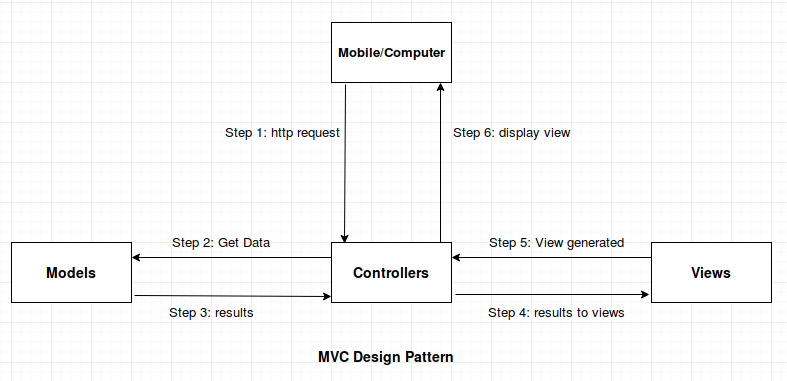
\includegraphics[width=1.0\columnwidth]{mvc}
\caption{MVC Design Pattern}
\label{fig:MVC Design Pattern}
\end{figure}

Model View Controller (MVC) is a software architectural pattern for implementing user interfaces. It divides a given application into three interconnected parts in order to separate internal representations of information from the ways that information is presented to and accepted from the user.The MVC design pattern decouples these major components allowing for efficient code reuse and parallel development.


\section{Django MTV Design Pattern}
According to the Django Book, Django follows the MVC pattern closely enough to be called an MVC framework.Django has been referred to as an MTV framework because the controller is handled by the framework itself and most of the excitement happens in models, templates and views.

\begin{figure}[htp]
\center
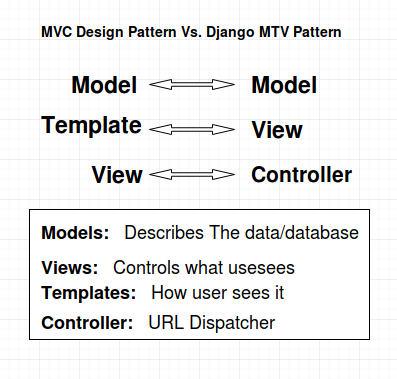
\includegraphics[width=0.5\columnwidth]{mvcMtv}
\caption{MVC Vs Django MTV}
\label{fig:MVC Vs Django MTV}
\end{figure}

\section{Django KodeFork Project}
Django project is a way to develop a web portal using Django framework and python as server side language. For example project \textbf{kodefork} is started using
\begin{minted}
[frame=lines,framesep=2mm,baselinestretch=1.2,]
{python}
django-admin startproject kodefork
\end{minted}

It creates a kodefork project directory. Inside the project directory there is an initial \textbf{kodefork app} and \textbf{manage.py} file.\\

\subsection{kodefork app}
It has mainly \textbf{settings.py} file and \textbf{urls.py} file.
\begin{itemize}
    \item\textbf{settings.py file:} This file contains all the basic settings for the project. It contains setting mainly for:
        \begin{itemize}
            \item Base Directory
            \item Secret Key
            \item Allowed Hosts
            \item Installed Apps
            \item Root URL
            \item Templates
            \item WSGI Application
            \item Databases
            \item Authorization Password Validators
            \item Language Code
            \item Time Zone
            \item Static Root and Static URL
            \item Media Root and Media URL
            \item Accounts
            \item Emails
        \end{itemize}
        
    \item\textbf{urls.py file:}This file contains starting urls for all apps. After start of url is matched, it then calls the urls.py of that particular app to handle subsequent request.For example:
    \begin{minted}
    [frame=lines,framesep=2mm,baselinestretch=1.2,]
    {python}
    # URL Handler for the website
    from django.conf.urls import url,include
    from django.contrib import admin
    admin.autodiscover()   
    urlpatterns = [
        url(r'^admin/', admin.site.urls),    
        url(r'^', include('main.urls')),   
        url(r'^learn/', include('learn.urls')),
        url(r'^questions/', include('questions.urls')),
    ]
    \end{minted}   
    
\end{itemize}

\subsection{manage.py file}
manage.py file is used for carrying management related tasks on the project. After starting project we need to create initial migrations and migrate it to database using:
\begin{minted}
[frame=lines,framesep=2mm,baselinestretch=1.2,]
{python}
# Make initial migrations
python manage.py makemigrations
# Make changes to database
python manage.py migrate
\end{minted}

Above commands creates an automatic admin portal with \textbf{users} model and \textbf{groups} model. This can be viewed by first creating a \textbf{superuser} for this project. For example create super user \textbf{astikanand}:
\begin{minted}
[frame=lines,framesep=2mm,baselinestretch=1.2,]
{python}
# Create Super User
python manage.py createsuperuser
\end{minted}
After Creating superuser start the management server like this
\begin{minted}
[frame=lines,framesep=2mm,baselinestretch=1.2,]
{python}
# In localhost
python manage.py runserver 0.0.0.0:8000
# In live server
Web server runs the project, in this project nginx server
\end{minted}

View the project in browser using:
\begin{minted}
[frame=lines,framesep=2mm,baselinestretch=1.2,]
{python}
# In localhost
http://localhost:8000
# In live server, for this project
http://www.kodefork.com
\end{minted}

\newline
Visit the admin portal now:
\begin{minted}
[frame=lines,framesep=2mm,baselinestretch=1.2,]
{python}
# In localhost
http://localhost:8000/admin
# In live server, for this project
http://www.kodefork.com/admin
\end{minted}

Now to implement any new feature we make an app for it and register it in \textbf{INSTALLED APPS}.

\section{Django Apps}
Every feature in django project is implemented using django apps. An app for example \textbf{ learn app} can be created by
\begin{minted}
[frame=lines,framesep=2mm,baselinestretch=1.2,]
{python}
python manage.py startapp learn
\end{minted}

\textbf{Every app has following items:}
\subsection{migrations directory}
It keeps track of all the migrations or changes that occur on models. After making any change on models inside an app, new migrations are generated using
\begin{minted}
[frame=lines,framesep=2mm,baselinestretch=1.2,]
{python}
python manage.py makemigrations learn
\end{minted}
basically this generates the sql query. After this we need to make changes to database or sync the database with changes. It is done using
\begin{minted}
[frame=lines,framesep=2mm,baselinestretch=1.2,]
{python}
python manage.py migrate learn
\end{minted}
once this is done, we can see that changes get reflected in datatabase model or models.

\subsection{static directory}
It keeps all the static files, like css, js, basic images and serves to the html templates to display pages. Other images and media files are served using Media Server of Django. Static files are served by first including it on top of html file using 

\begin{minted}
[frame=lines,framesep=2mm,baselinestretch=1.2,]
{python}

\end{minted}

and then by making a reference to it

\begin{minted}
[frame=lines,framesep=2mm,baselinestretch=1.2,]
{python}
href=""
\end{minted}


\subsection{templates directory}
It contains all the html files. Once the function inside views.py collects data requested from appropriate model, it send that data to html template file. Inside templates directory basically we have one base.html which is kind of skeleton for every html file. The base.html is inherited on top of every other html file of that app using

\begin{minted}
[frame=lines,framesep=2mm,baselinestretch=1.2,]
{python}

\end{minted}

We make something like containers in base.html file for everything that is to be filled by other html files. For example:

\begin{minted}
[frame=lines,framesep=2mm,baselinestretch=1.2,]
{python}

\end{minted}

In every page we have different content and hence we make container or block for it in base.html file. The data which comes from views to template using a python dictionary is displyed in html file using a template language called \textbf{jinja}

\subsection{urls.py file}
It contains a number of regular expressions to match a url and calls appropriate view function in views.py. For an example

\begin{minted}
[frame=lines,framesep=2mm,baselinestretch=1.2,]
{python}
# URL Handler for the learn
from django.conf.urls import url
from . import views
app_name = 'learn'
urlpatterns = [
    url(r'^$', views.subjects, name='learnhome'),
    
    url(r'^(?P<subjectslug>[A-Za-z-_.]+)/$', views.chapters,
    name='learnsubject'),
    
    url(r'^(?P<subjectslug>[A-Za-z-_.]+)/(?P<categoryslug>
    [A-Za-z-_.]+)/(?P<chapterslug>[A-Za-z-_.]+)/$', 
    views.topics, name='learnchapter'),
    
    url(r'^(?P<subjectslug>[A-Za-z-_.]+)/(?P<categoryslug>
    [A-Za-z-_.]+)/(?P<chapterslug>[A-Za-z-_.]+)/
    (?P<topicslug>[A-Za-z-_.]+)/$',
    views.contents, name='learntopics'),
]
\end{minted}

\subsection{views.py file}
It contains all the views function which controls what user sees, after url make a call to appropriate view function in views.py. The function if necessary collects data from model/models and stores in a dictionary and sends it to appropriate templates file. Templates file after receiving data display it in html using \textbf{jinja} template. For an example

\begin{minted}
[frame=lines,framesep=2mm,baselinestretch=1.2,]
{python}
# Takes a request and send back the response
from django.http import Http404
from django.shortcuts import render,get_list_or_404,
get_object_or_404
from django.db.models import Count
from . models import *

# Get the contents from a particular topic
def contents(request, subjectslug, categoryslug, chapterslug, 
topicslug):

    subject =get_object_or_404(Subject,subjectSlug=subjectslug)
    
    chapter = get_object_or_404(Chapter,subject__subjectSlug=
    subjectslug,chapterSlug=chapterslug)
    
    topics = Topic.objects.filter(subject__subjectSlug=
    subjectslug,category__categorySlug=categoryslug,
    chapter__chapterSlug = chapterslug).order_by('topicNumber')
    
    if not topics:
        raise Http404

    contents = get_object_or_404(Topic, subject__subjectSlug=
    subjectslug,category__categorySlug=categoryslug,
    chapter__chapterSlug = chapterslug,topicSlug=topicslug)

    act = request.path.split('/')[5]
    
    url = '/learn/'+subjectslug+'/'+categoryslug
    
    #create a python dictionary to sent it to html template
    context = { 'subject':subject, 'chapter': chapter, 
    'topics': topics,'contents': contents, 'act':act,
    'url': url }
    
    return render(request, 'learn/contents.html', context)

\end{minted}

We can also write some class based views instead of normal views function. Django also provides some generic class based views.
\begin{itemize}
    \item django.views.generic.ListView
    \item django.views.generic.DetailView
    \item django.views.generic.TemplateView
    \item django.views.generic.edit.FormView
    \item django.views.generic.edit.CreateView
    \item django.views.generic.edit.UpdateView
    \item django.views.generic.edit.DeleteView
\end{itemize}

\textbf{We can use class based views like this.}
\begin{minted}
[frame=lines,framesep=2mm,baselinestretch=1.2,]
{python}
class UserUpdate(LoginRequired,AuthorRequiredMixin,UpdateView):
    model = Profile
    
    template_name = 'users/profile_update.html'
    
    fields = ['gender','profilepic','designation','about',
    'address','website','facebookprofile','twitterprofile',
    'githubprofile','linkedinprofile']
    
    pk_url_kwarg = 'userid'

    def get_success_url(self):
        people = self.get_object()
        
        successurl = '/users/'+str(people.pk)+'/'+
        str(people.user)
        
        return successurl
\end{minted}

The generic views is used to directly create, update or delete entry inside model by creating a form at template specified in it.


\subsection{models.py file}
It contains a collection of models which is same as tables in normal sql language. Every model has several fields denoting entities. For example

\begin{minted}
[frame=lines,framesep=2mm,baselinestretch=1.2,]
{python}
from django.db import models
from ckeditor_uploader.fields import RichTextUploadingField
from django.template.defaultfilters import slugify
from django.core.urlresolvers import reverse
from smart_selects.db_fields import *


# Models for learn section
class Subject(models.Model):
    subjectNumber = models.IntegerField(default=1)
    
    subjectName = models.CharField(max_length=500)
    
    subjectSlug = models.SlugField(editable=False)
    
    subjectDescription = models.TextField(null=True)
    
    subjectKeywords = models.CharField(max_length=500,null=True)
    
    subjectIcon = models.ImageField(upload_to=
    'uploads/learn/%Y/%m/%d/', null=True, blank=True)
    
    subjectThumbnail = models.ImageField(upload_to=
    'uploads/learn/%Y/%m/%d/', null=True, blank=True)
    
    subjectTwitterImage = models.ImageField(upload_to=
    'uploads/learn/%Y/%m/%d/', null=True, blank=True)
    
    subjectOpengraphImage = models.ImageField(upload_to=
    'uploads/learn/%Y/%m/%d/', null=True, blank=True)


    def save(self):
        if not self.id:
            self.subjectSlug = slugify(self.subjectName)

        super(Subject, self).save()

    def __str__(self):
        return self.subjectName
\end{minted}


In above model in \textbf{ImageField} uploadto  is used to a directory as per upload Year, month and date and uploads image, if name conflicts it renames it and then uploads.\textbf{SlugField()} and \textbf{slugify()} function is used to create slug, 
which helps in creating clean urls. For example:\\

\emph{ if subjectname = 'Data Structures' its generated slug will be \\ slug='data-structures'}\\

Once any changes is made in models, new migrations is created and it is migrated to make changes in database as specified earlier.

\subsection{admin.py file}
This file is used to register models inside admin. Once model is registered it shows up in admin panel of project. For example:

\begin{minted}
[frame=lines,framesep=2mm,baselinestretch=1.2,]
{python}
from django.contrib import admin
from .models import Subject, Category, Chapter, Topic

admin.site.register(Subject)
admin.site.register(Category)
admin.site.register(Chapter)
admin.site.register(Topic)
\end{minted}

\subsection{forms.py file}
This file contains all forms related to that app. Forms can be created by 2 types.\\

Firstly by using simple \textbf{forms.form}

\begin{minted}
[frame=lines,framesep=2mm,baselinestretch=1.2,]
{python}
from django import forms

class MessageForm(forms.Form):
    name = forms.CharField(max_length=100)
    email = forms.EmailField()
    subject = forms.CharField(max_length=100)
    message = forms.TextField()
    
\end{minted}

and secondly it can be created using \textbf{forms.ModelForm}

\begin{minted}
[frame=lines,framesep=2mm,baselinestretch=1.2,]
{python}
from django import forms
from . models import Message

class MessageForm(forms.ModelForm):

    class Meta:
        model = Message
        fields = ['name','email','subject','message']
\end{minted}
Form is then processed and saved using appropriate function in views.py.

\section{Working of Django app}
\begin{figure}[htp]
\center
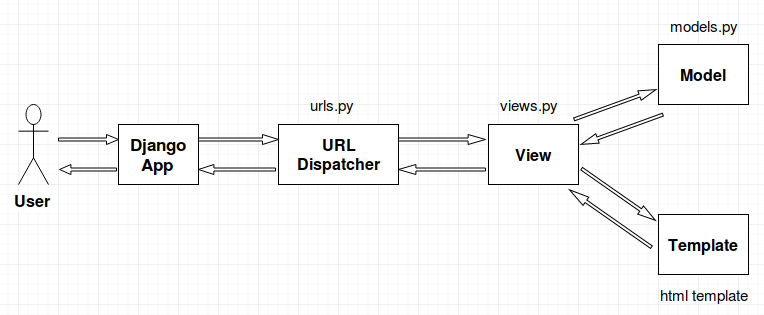
\includegraphics[width=1.0\columnwidth]{djangoapp}
\caption{Working of Django App}
\label{fig:Working of Django App}
\end{figure}

Firstly request made by user using url(regular expression) hits the appropriate django  app, then it checks the urls matching regular expression and then appropriate url is dispatched. The dispatched url calls an appropriate view function in views.py. View function in views.py then collects data from model or models if needed and stores it in a dictionary. It then sends the dictionary to html template file. The data inside the dictionary is displayed in html template file using \textbf{jinja} template. This html file is then displayed to user.\\
\textbf{Almost every feature in django project is implemented using an abstract app and all these apps works in similar fashion as described above.}

\chapter{Design}
\section{Software Description}
\subsection{Perspective}
The purpose of this portal is to provide people with an effective learning portal where they can learn computer science subjects or technologies using section and topic wise tutorials. It also provides them conceptual and competition problem for every topic. This portal also provides question answering community, where people can ask and answer questions. This portal provides articles on recent topics and technologies and also gives people an option to write and publish their own articles.This portal provide an online editor and compiler for various programming languages where people can write their code, compile and run it.


\subsection{Features}
The website is designed using django framework in which every major section is implemented by creating new apps. So, this portal has also many apps and every app has its own features which is described below. One of main feature of this portal is responsiveness. The portal is designed in such a way that it is an all device portal. The portal get adjusted to all standard width devices automatically.

\begin{itemize}
    \item \textbf{main app}
    \begin{itemize}
         \item Displays homepage when user enters portal by visiting the url \emph{www.kodefork.com}
         \item 
    \end{itemize}
    
\end{itemize}


\chapter{Design}





The development of a Natural Language Interface to Database (NLIDB) System comprises of the following two systems\cite{eight}:

\begin{itemize}

\item \textbf{Linguistic component}\\
The objective of this component is to translate natural language input SQL query and hence generate the data asked by querying the database.

\item \textbf{Database component}\\
This component performs the Database Management functions. Where a lexicon is used to map the words from the natural query to database relation names, attribute names and some constraint relationship (eg. Foreign Key - Primary Key relationship). Generated parse tree for natural language query is then mapped to database objects using semantic interpreter with the help of lexicon. And a natural language generator is used to parse the resultant parse tree to generate a natural language response. Questions entered in natural language translated into a statement in a formal query language. Once the statement unambiguously formed with the help of user interaction. Then query is given to database management system and after processing desired data is generated.

\begin{figure}[htp]
\center
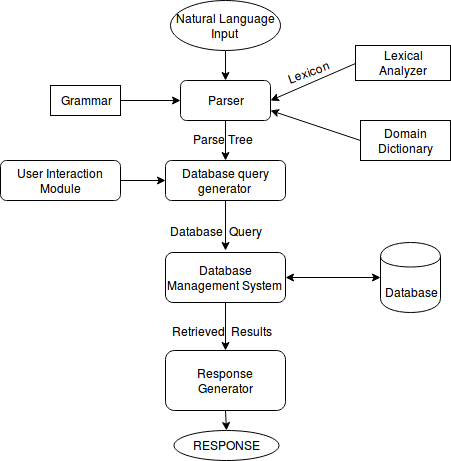
\includegraphics[width=0.5\columnwidth]{newHLL}
\caption{High level design.}
\label{fig:High level design}
\end{figure}

\item The natural language input is first processed syntactically by the parser. A parse tree is generated by parser using syntax rules from grammar. User interaction is used to remove any ambiguity in query input.

\item Then using semantic interpreter parse tree is transformed in an intermediate logic query. The semantics rule computes the logic expression of left nodes of the syntax rule, as a function of the logic expressions of the right-hand side of the syntax rule. The logic expressions corresponding to words are declared in the lexicon.\cite{two}

\item The semantic interpreter also consults a world model, that describes the structure of the surrounding world. Typically, the world model contains a hierarchy of classes of world objects, and constraints on the types of arguments each logic predicate may have.\cite{two}

\item The logic query generated by the parsing and semantic interpretation module, expresses the meaning of the user’s question in terms of logical, high-level concepts. Database query generator transforms logical to SQL query using mapping to database information.

\item Generated SQL query is given as input to underlying DBMS in order to retrieve requested data from database. DBMS queries the database and generated response is passed to the response generator. Responsibility of the response generator is to provide fetched result from database to user.

\item \textbf{Generation of the Domain Dictionary} \\
Dictionaries used by existing NLIDBs are created manually or semi-automatically. We can automate the generation of the domain dictionary from a synonym dictionary and the database metadata with the help of some linguistic processing.

\begin{figure}[ht]
\center
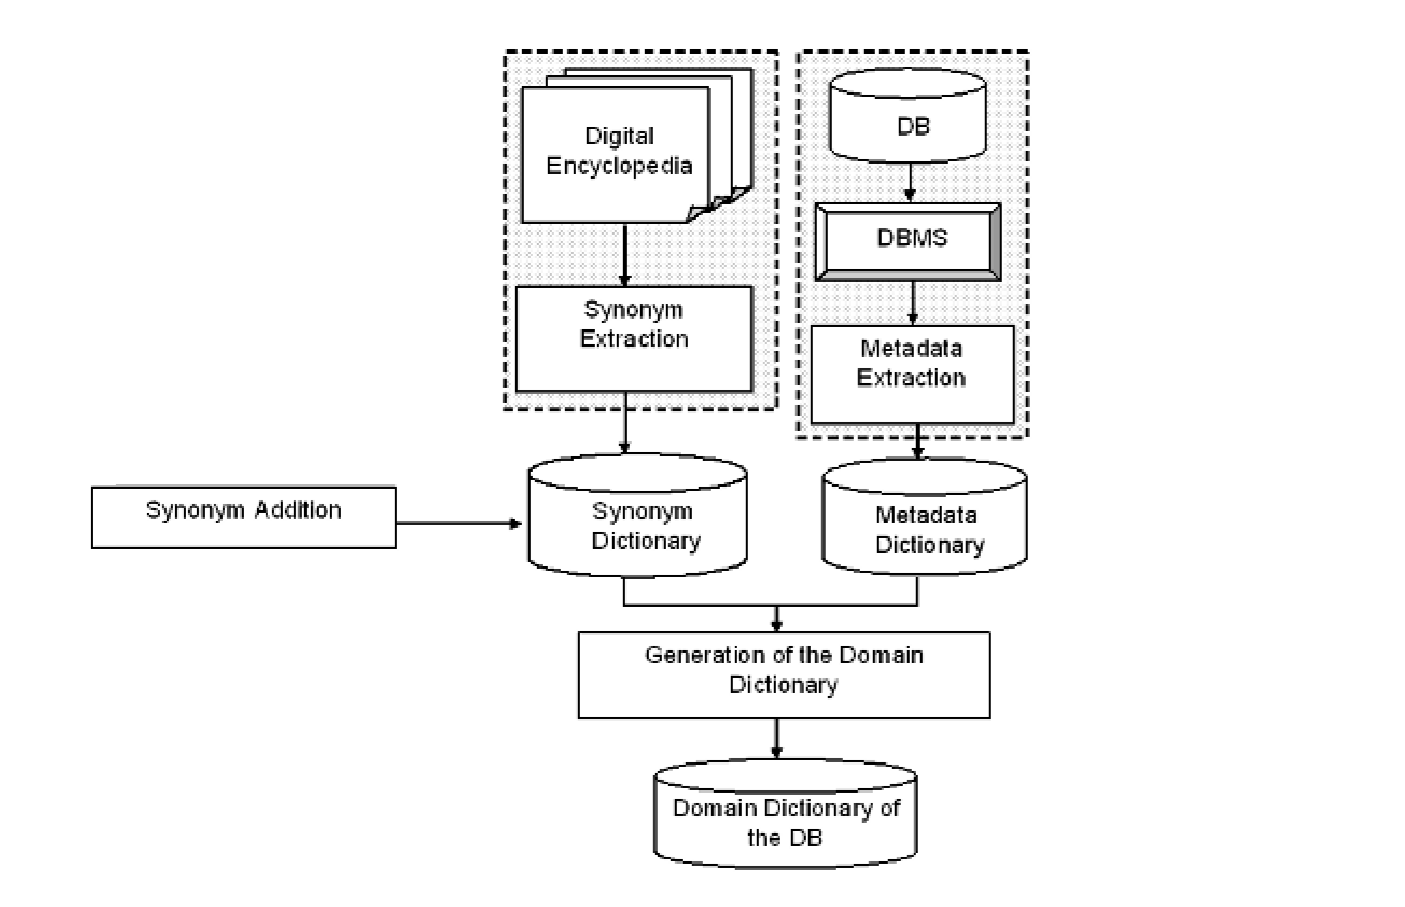
\includegraphics[width=1\columnwidth]{Dictionary}
\caption{Generation of domain dictionary}
\label{fig:Generation of domain dictionary}
\cite{five}
\end{figure}

\item \textit{Synonym dictionary}\\
A general synonym dictionary can be extracted from a digital encyclopedia. Encyclopedia contains synonyms and antonyms of thousands of the words. This dictionary can be used for most domains to better interpret query. WordNet\cite{aaa} is an example for such encyclopedia which can also be used for this purpose.

\item \textit{Metadata dictionary}\\
Queries to database are restricted to database domain. So a dictionary generated from database can be used for better mapping of natural language query to database relations and attributes.  The metadata dictionary store database information such as number of tables, number of columns, and its location. Additionally, for each table it stores the name of each column along with its data type and description, which contains primary key and foreign key information used to translate a complex query using join operations.

\item \textit{Domain dictionary}\\
For automatic generation of the domain dictionary, the description of each column from the metadata dictionary is processed to obtain the lemma and the part of speech (POS) of each word in the description.
\end{itemize}



\chapter{Implementation}


The various stages in the implementation of the proposed system are as\\ follows:\\

\section{User Interface}
First the user selects the database of choice. Now the user can input the natural language query in the user interface. The user interface is meant so that the user can aid the system in query translation. The user plays an integral role in node mapping, discussed in section \ref{mapping}.
\section{Schema Graph}
The database schema taken from the underlying database is represented as follows:
\begin{itemize}
\item There are two types of nodes. 
\subitem{Relation Nodes(RN) : to represent the relations} 
\subitem{Attributes Nodes(AN) : to represent the attributes of the relations}
\item Similarly, there are two types of edges. 
\subitem{Relation Edges : to represent the foreign key-primary key relationship.} 
\subitem{Attributes Edges : to represent the attributes of the relations. For every RN there is a edge from it to all the AN which represents the attribute of the corresponding relation.}
\end{itemize}

\begin{algorithm}[Q]
\SetAlgoLined




\SetKwInOut{Input}{input}\SetKwInOut{Output}{output}
\Input{A Database \textbf{db} }
\Output{Schema Graph \textbf{S(V,E)} representing \textbf{db}}
\BlankLine




\textbf{dbSchema} $\leftarrow$ \emph{extract schema from } \textbf{db}

\textbf{keyRelations} $\leftarrow$ \emph{ extract primary key - foreign key relations from } \textbf{dbSchema} 

\textbf{tables} $\leftarrow$ \emph{ extract table names from } \textbf{dbSchema} \;

\ForEach{ \emph{tableName} \in \textbf{tables}}{
    
    \textbf{\emph{columns}}\emph{[tableName]} $\leftarrow$  \emph{extract all attributes of tableName from } \textbf{dbSchema}
 
}

\textbf{S(V,E)} $\leftarrow \phi$

\ForEach{ \emph{tableName} \in \textbf{tables}}{
    \textbf{S(V)}.add(makeRelationNode(tableName))
    
  

}


\ForEach{ \emph{(FK,PK)} \in \textbf{tables}}{
    \textbf{S(E)}.addDirectedEdge(FK, PK)
}

\ForEach{colName \in \textbf{columns}[tableName]}{
        \textbf{S(V)}.addAttributeNode(colName)
    }

\ForEach{ \emph{tableName} \in \textbf{tables}}{

    \ForEach{colName $\in$ \textbf{columns}[tableName]}{
        \textbf{S(E)}.addDirectedEdge(tableName, colName)\\
        \textbf{\emph{sampleData}}\emph{[columnName]} $\leftarrow$ \emph{extract \emph{t} samples from columnName of tableName using } \textbf{db}  
    }
     
}
\textbf{Return} \textbf{\emph{S(V,E)}}
 \caption{Schema Graph Generation}
\end{algorithm}

\newpage

\section{Parse tree}
The natural language input is parsed using Stanford Parser.\cite{ten} This parse tree is used to understand the structure of the input. This parse tree has the following different type of nodes,


The stanford parser gives a tree of words. For each of these words in the parse tree we create a corresponding node in our parse tree with the word as its value and the tree structure is maintained. 


\begin{figure}[htb]
\centering
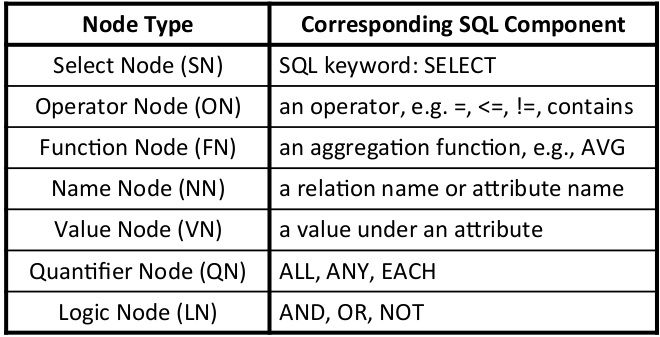
\includegraphics[scale=0.55]{nodes} % e.g. insert ./image for image.png in the working directory, adjust scale as necessary
\caption{Parse tree nodes}
\label{fig:aa} % insert suitable label, this is used to refer to a fig from within the text as shown above
\end{figure}


The figure \ref{fig:vv} is an example of a parse tree generated by the stanford parser,
\newpage


\begin{figure}[htb]
\centering
\includegraphics[scale=0.5]{pt} % e.g. insert ./image for image.png in the working directory, adjust scale as necessary
\caption{Parse tree for the NL query}
\label{fig:vv} % insert suitable label, this is used to refer to a fig from within the text as shown above
\end{figure}

\section{SQL Query Grammar }
The figure \ref{fig:grammara} shows is the grammar used to represent an SQL query in this project,

\begin{figure}[htb]
\centering
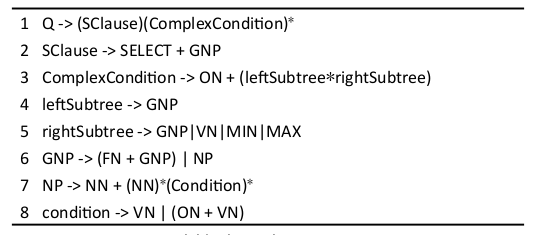
\includegraphics[scale=0.45]{./gram} % e.g. insert ./image for image.png in the working directory, adjust scale as necessary
\caption{Grammar for a SQL query}
\label{fig:grammara} % insert suitable label, this is used to refer to a fig from within the text as shown above
\cite{eleven}
\end{figure}

\newpage
In Figure \ref{fig:grammara},
+ represents a parent-child relationship.
* represents a sibling relationship.
One Query (Q) can must have one SClause and zero or more ComplexConditions.
A ComplexCondition must have one ON, with a leftSubtree and a rightSubtree.
An NP is: one NN (since an SQL query has to select at least one attribute), whose children are multiple NNs and Conditions. (All other selected attributes and conditions are stacked here to form a wide "NP" tree.)\cite{eleven}\\
All the valid parse trees should be in accordance to this grammar. So our aim is to rearrange the parse tree so that it follows the grammar.

\section{Node mapping}\label{mapping}
The identification of select node, operator
node, function node, quantifier node and logic node is independent of the database being queried.
Name nodes and value nodes correspond to
the meta-data and data, respectively, which entirely depend
on the database being queried.
When a parse tree node has multiple candidates for mapping it into particular type of node then our system returns multiple candidate mappings for the user to choose from. Also the user may also specify that some words are meaningless or unknown to him. Such nodes have to be removed from the tree.



\begin{algorithm}[H]
\SetAlgoLined




\SetKwInOut{Input}{input}\SetKwInOut{Output}{output}
\Input{A parse tree from stanford parser \textbf{PT} }
\Output{Mapped Parse Tree}
\BlankLine

\ForEach{ \emph{node} $\in$ \textbf{PT}}{\If{node.value $\in$ keywords}{ 
        node.type = node.value \\
        \emph{continue}
    }
    
    \textbf{choicesToMap} $\leftarrow$ \emph{calculateChoices(node.value)}\\
    
    \textbf{userChoice} $\leftarrow$ ask user to choose from a set of choices $\in$ \textbf{choicesToMap } ordered in decreasing value of relevance \\
    node.type = userChoice
    
    
}


\textbf{Return} \textbf{PT}


 \caption{Node Mapping}
\end{algorithm}

\begin{algorithm}[Y]
\SetAlgoLined




\SetKwInOut{Input}{input}\SetKwInOut{Output}{output}
\Input{A parse tree node \textbf{node}, \textbf{schema graph S}, \textbf{WordNet}  }
\Output{List of mapping choices}
\BlankLine

\textbf{choices} $\leftarrow$ ()\\
\ForEach{colName $\in$ \textbf{S.columns}}{
    \emph{score $\leftarrow$ \textbf{WordNet.similarity}(colName, \textbf{node.value})}
    \emph{\textbf{choices}.append((colName,score,NN))}
}

\ForEach{tableName \in \textbf{S.tables}}{
    score = $\leftarrow$ \textbf{WordNet.similarity}(tableName, \textbf{node.value})
    \textbf{choices}.append((tableName,score,NN))
}

\ForEach{colName \in \textbf{S.columns}}{
    \textbf{score} $\leftarrow$ \emph{1}\\
    \ForEach{\emph{data} $\in$ \textbf{S.sampleData}[columns]}{
        \textbf{score}*=\textbf{WordNet.similarity}(node.value,data)
        \textbf{choices}.append((colName,score,NV))
    }
    
}
\textbf{Return} \textbf{\emph{choices}}
 \caption{calculateChoices()}
\end{algorithm}

The node mapping is done with the help of user interaction. The user selects the node type from a list of possible types ordered in decreasing order of its score. Score of type for a particular node is calculated by finding out the similarity between them. The similarity measure used is from WordNet. 




\begin{figure}[htb]
\centering
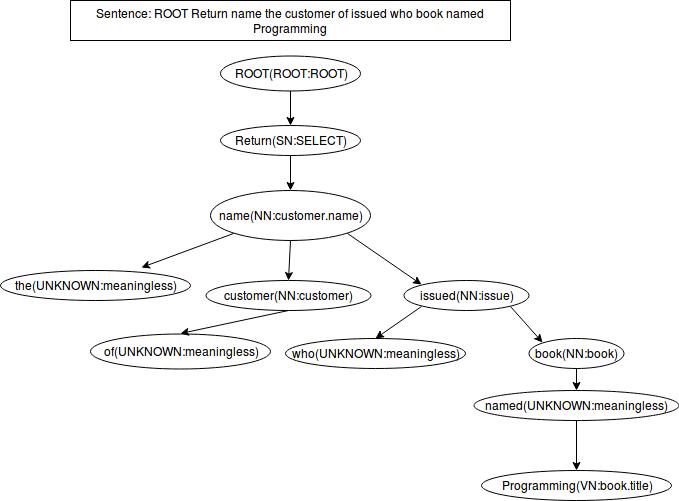
\includegraphics[scale=0.45]{./map} % e.g. insert ./image for image.png in the working directory, adjust scale as necessary
\caption{Parse after node mapping }
\label{fig:grammar} % insert suitable label, this is used to refer to a fig from within the text as shown above
\end{figure}




\begin{figure}[htb]
\centering
\includegraphics[scale=0.45]{./rem} % e.g. insert ./image for image.png in the working directory, adjust scale as necessary
\caption{Parse after removing meaningless nodes}
\label{fig:grammar} % insert suitable label, this is used to refer to a fig from within the text as shown above
\end{figure}







\section{Rearrangement of parse tree}
After all the nodes of the parse tree is mapped,the tree can be understood by the system. But linguistic parse tree generated from a parser may be incorrect as natural language sentences often have complex structures and also such parse trees may not be completely in adherence of the SQL query grammar. So the parse tree has to be rearranged to get a suitable tree.\\








\begin{algorithm}[J]
\SetAlgoLined
\SetKwInOut{Input}{input}\SetKwInOut{Output}{output}


\Input{A parse tree \textbf{parseTree}  }
\Output{A list of relevant parse trees}


\BlankLine

\textbf{results} $\leftarrow$ \phi\\
\textbf{PriorityQ} $\leftarrow$ \phi\\
PriorityQ.insert(\textbf{parseTree})\\
\While{PriorityQ $\ne$ \phi}{
    Ptree = PriorityQ.remove()\\
    treeList = adjust(Ptree)\\
    \ForEach{tree $\in$ \emph{treeList}}{
        \If{tree.edit \textless t }{
            tree.edit += 1\\
            \If{evaluateScore(tree) $\ge$ evaluateScore(Ptree)}{
                PriorityQ.insert(tree')\\
                \If{tree is valid}{
                    \textbf{results}.append(tree)
                }
            }
        }
    }
}
\textbf{Return} \textbf{\emph{results}}

 \caption{Tree Rearrangement}
\end{algorithm}







\begin{algorithm}[K]
\SetAlgoLined
\SetKwInOut{Input}{input}\SetKwInOut{Output}{output}


\Input{A parse tree \textbf{parseTree}  }
\Output{A list parse trees }


\BlankLine

\textbf{adjustedTrees} $\leftarrow$ \phi\\

\ForEach{\emph{node} $\in$ \textbf{\emph{parseTree}}}{
    \ForEach{child in \emph{node}}{
        \textbf{\emph{adjustedTrees}}.add(swap \emph{node} and child)\\
        \textbf{\emph{adjustedTrees}}.add(make \emph{node} its sibling)\\
        \textbf{\emph{adjustedTrees}}.add(make siblings the child of \emph{node})\\
        \textbf{\emph{adjustedTrees}}.add(swap \emph{node's} children)\\
    }
    
}

\textbf{Return} \textbf{\emph{adjustedTrees}}

 \caption{adjust()}
\end{algorithm}





\begin{figure}[htb]
\centering
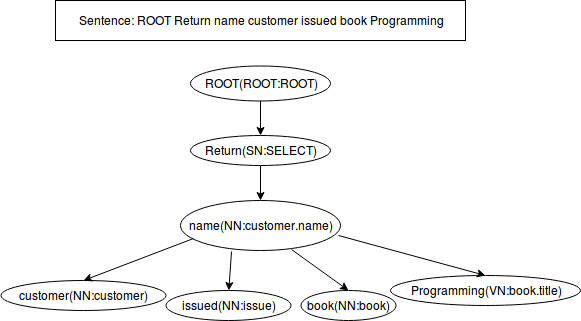
\includegraphics[scale=0.45]{./tran} % e.g. insert ./image for image.png in the working directory, adjust scale as necessary
\caption{Best rearranged parse tree for the query}
\label{fig:grammar} % insert suitable label, this is used to refer to a fig from within the text as shown above
\end{figure}

The basic idea is to move sub-trees to edit the parse tree until it is syntactically correct according to the grammar defined.Each time, we use the move function we  generate all the possible parse trees in one
sub-tree move operation. The number of parse trees grows exponentially with the number of edits. To fasten the process,
 each new generated parse tree is evaluated and
 bad parse trees directly filtered out. We also set a parameter as the
maximum number of edits approved. Our system
records all the valid parse trees appeared in the reformulation process and returns the top k of them so that the user can choose from them.\\
Now to rate each of the generated parse trees in the method above we set the score of the parse tree as the negative of the number of invalid nodes it has. A node is said to be invalid if that node does not follow the grammar defined for SQL queries.



\section{SQL query generation}
Last step in our process is to generate SQL query from query tree. Since the parse tree now adheres to the SQL grammar the we have defined the translation is done directly according to it. The schema element mapped by the node which has similarity between label and schema element name, under the SELECT node is added
to the SELECT clause. Each value node is transformed to a selection condition and added to the WHERE clause. Finally, a foreign key-primary key
join path is generated, according to the schema graph, to
connect each nodes in the select clause and its neighbors. Such an foreign key-primary key join path is translated into a series of foreign key-primary key join conditions and all the schema elements in the foreign key-primary key join path are added to the FROM clause.\cite{eleven}





\chapter{Experimental Results}

The system is tested against a library database. The system gives satisfactory results for both simple queries and complex queries with foreign key-primary key relationships along with aggregate functions. As the implementation only incorporates single word attributes, testing it for complex database is difficult. A syntactically correct SQL query is almost always generated for a correctly mapped parse tree. The figure \ref{fig:schema} represents the schema for the library database,\\

\begin{figure}[htb]
\centering
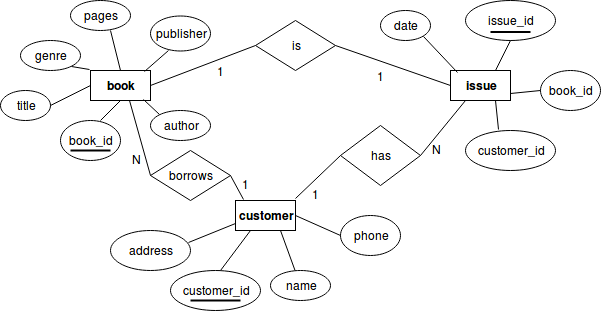
\includegraphics[scale=0.55]{./er} % e.g. insert ./image for image.png in the working directory, adjust scale as necessary
\caption{Schema for library database}
\label{fig:schema} % insert suitable label, this is used to refer to a fig from within the text as shown above
\end{figure}




\section{Simple queries}

\begin{enumerate}
\item \textbf{Input: Give me every book.}\\
\textbf{Query:}\\SELECT book FROM book;\\
\textbf{Output:}\\
('(1,Heartless,Stephens,Romantic,123,Martin)',)\\
('(2,King,Khan,Action,342,Khan)',)\\
('(3,Lord,Bose,History,233,BPB)',)\\
...\\
('(25,Beautiful,Oldman,Romantic,389,McGrawHill)',)\\
('(26,Mind,Narayana,Science,612,Scifi)',)\\
('(27,Tempest,Narayana,Science,231,Scifi)',).


\item \textbf{Return all book titles and pages.}\\
\textbf{Query:}\\SELECT book.title, book.pages FROM book;\\
\textbf{Output:}\\
('Heartless', 123), ('King', 342), ('Lord', 233),\\
......,\\
,('Beautiful', 389),('Mind', 612),('Tempest', 231).

\item \textbf{
Fetch all customer name and address.}\\
\textbf{Query:}\\SELECT customer.name, customer.address FROM customer;\\
\textbf{Output:}\\
('John', 'Delhi'),('Adam', 'Delhi'),('Kishor', 'Mumbai')\\
...\\
('Suraj', 'Delhi'),('Chaitanya', 'Raigarh'),('Neeraj', 'Raipur').

\item \textbf{Fetch all book whose author is Amrish.}\\
\textbf{Query:}\\SELECT book FROM book WHERE book.author = 'Amrish';\\
\textbf{Output:}\\
('(21,Shiva,Amrish,Drama,543,Tripathi)',),\\
('(22,Shiva2,Amrish,Drama,323,Tripathi)',),\\
('(23,Shiva3,Amrish,Drama,464,Tripathi)',).

\item \textbf{Return name of customers who are not living in Mumbai.}\\
\textbf{Query:}\\
SELECT customer.name FROM customer\\
WHERE customer.address != 'Mumbai';\\
\textbf{Output:}\\
('John',),('Adam',),('Kamlesh',),('Akshay',),('Jobin',),('Nirant',),\\
('Anurag',),('Bhupendra',),('Harshit',),('Balmukund',),('Vipin',),('Mayank',)\\
('Anand',),('Astik',),('Ashok',),('Prabhav',),('Suraj',),('Chaitanya',),('Neeraj',)\\

\item \textbf{Return count of customer we have.}\\
\textbf{Query:}\\SELECT COUNT(customer) FROM customer;\\
\textbf{Output:}\\ (22)

\item \textbf{Return number of books.}\\
\textbf{Query:}\\SELECT COUNT(book) FROM book;\\
\textbf{Output:}\\ (27)

\item \textbf{Return average pages in books.}\\
\textbf{Query:}\\SELECT AVG(book.pages) FROM book;\\
\textbf{Output:}\\ ('424.0370370370370370')

\end{enumerate}

\section{Complex queries}

\begin{enumerate}
\item \textbf{Return name of customer who issued a book named Inception.}\\
\textbf{Query:}\\SELECT issue, customer.name\\
FROM customer, book, issue\\
WHERE book.book\_id = issue.book\_id\\ 
AND customer.customer\_id = issue.customer\_id\\ 
AND book.title = 'Inception' \\
AND issue.book\_id = book.book\_id;\\
\textbf{Output:}\\ ('(16,19,12,2009)', 'Vishal')

\item \textbf{Print all book published by Tripathi publications and whose genre is Drama.}\\
\textbf{Query:}\\SELECT book FROM book \\
WHERE book.genre = 'Drama' AND book.publisher = 'Tripathi';\\
\textbf{Output:}\\
('(21,Shiva,Amrish,Drama,543,Tripathi)',),\\
('(22,Shiva2,Amrish,Drama,323,Tripathi)',),\\
('(23,Shiva3,Amrish,Drama,464,Tripathi)',)

\item \textbf{fetch all customers names  who issued Drama book of Amrish.}\\
\textbf{Query:}\\SELECT issue, customer.name \\
FROM customer, book, issue\\
WHERE book.genre = 'Drama' AND book.book\_id = issue.book\_id \\
AND customer.customer\_id = issue.customer\_id \\
AND book.author = 'Amrish' \\
AND issue.book\_id = book.book\_id;\\
\textbf{Output:}\\
('(17,21,13,2011)', 'Vipin')\\
('(18,22,14,2015)', 'Mayank')\\
('(19,23,14,2013)', 'Mayank')\\

\item \textbf{fetch all customers names  who have not issued any book of Amrish.}\\
\textbf{Query:}\\SELECT customer.name, issue\\
FROM customer, book, issue\\
WHERE book.book\_id = issue.book\_id\\
AND customer.customer\_id = issue.customer\_id\\
AND book.author != 'Amrish'\\ 
AND issue.book\_id = book.book\_id;\\
('John', '(1,1,0,2015)'),('Adam', '(2,2,1,2016)'),('Adam', '(3,3,1,2015)')\\
....\\
('Bhupendra', '(14,16,9,2011)'),('Anurag', '(15,17,8,2010)'),('Vishal', '(16,19,12,2009)')\\

\item \textbf{fetch all customer who have issued any book before 2014.}\\
\textbf{Query:}\\SELECT customer\\
FROM customer, issue\\
WHERE customer.customer\_id = issue.customer\_id \\
AND issue.date < 2014;\\
\textbf{Output:}\\
('(2,Kishor,Mumbai,9147542363)',),('(3,Kamlesh,Raigarh,9148954662)',),\\
('(3,Kamlesh,Raigarh,9148954662)',),('(5,Jobin,Calicut,9147242426)',),\\
('(5,Jobin,Calicut,9147242426)',),('(8,Anurag,Raigarh,7332842921)',),\\
('(8,Anurag,Raigarh,7332842921)',),('(9,Bhupendra,Raipur,7332821414)',),\\
('(12,Vishal,Mumbai,7332842921)',),('(13,Vipin,Calicut,7332842923)',),\\
('(14,Mayank,Bilaspur,8522424413)',)

\item \textbf{Return customer name , address and issue date of book Shiva.}\\
\textbf{Query:}\\SELECT issue.date, customer.address, customer.name\\
FROM customer, book, issue\\
WHERE book.book\_id = issue.book\_id\\
AND customer.customer\_id = issue.customer\_id\\
AND book.title = 'Shiva'\\
AND issue.book\_id = book.book\_id;\\
\textbf{Output:}\\
(2011, 'Calicut', 'Vipin')

\item \textbf{Return count of customer we have who issued book before 2016.}\\
\textbf{Query:}\\SELECT COUNT(customer)\\
FROM customer, issue\\
WHERE customer.customer\_id = issue.customer\_id\\
AND issue.date < 2016;\\
Output: \\
(18)

\item \textbf{Return average pages in books by Amrish.}\\
\textbf{Query:}\\SELECT AVG(book.pages)\\
FROM book\\
WHERE book.author = 'Amrish';\\
\textbf{Output:}\\
('443.3333333333333333')\\


\item \textbf{print the number of customer do we have whose name is Anurag?}\\
\textbf{Query:}\\SELECT COUNT(customer)\\
FROM customer\\
WHERE customer.name = 'Anurag';\\
\textbf{Output:}\\
(1)

\item \textbf{Return name and phone of customer who lives in Delhi.}\\
\textbf{Query:}\\SELECT customer.phone, customer.name\\
FROM customer\\
WHERE customer.address = 'Delhi';\\
\textbf{Output:}\\
('9567843232', 'John')\\
('9547543332', 'Adam')\\
('73328423231', 'Harshit')\\
('7332323923', 'Astik')\\
('7332842867', 'Suraj')\\


\end{enumerate}


We tested the system on a total of 47 queries. The following is the tabulated results.

\begin{figure}[htb]
\centering
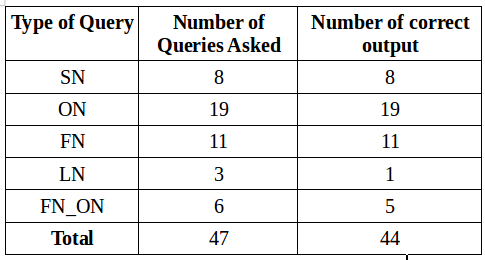
\includegraphics[scale=0.55]{./Results} % e.g. insert ./image for image.png in the working directory, adjust scale as necessary
\caption{Results}
\label{fig:grammar} % insert suitable label, this is used to refer to a fig from within the text as shown above
\end{figure}

\begin{itemize}
    \item SN : simple queries in which the query tree only has SN,NN,VN nodes
    \item ON : queries having SN,NN,VN and ON nodes  
    \item {FN : queries having SN,NN,VN and FN nodes  }
    \item {LN : queries having SN,NN,VN and LN nodes  }
    \item {FN\_ON : queries having SN,NN,VN,FN and ON nodes  }
\end{itemize}
    
    




\chapter{Conclusion and Future Work}

We have designed and implemented a natural language query
interface for databases which is interactive. Given a natural language
input we first translate it into a SQL statement and
then evaluate it against the underlying relational database. To achieve better output and accuracy the system shows each step of transformation of input to the user. If there are ambiguities, then for each ambiguity, the system outputs multiple top ranked interpretations so that the user can choose from them. The query mechanism described in this report has been implemented and the actual user experience has been gathered. While using the system the users are
able to query tasks satisfactorily.\\
In our current implementation we have only handled cases where database attributes are single words. It has to be enhanced so that we can use multiple word attribute data. A better scoring algorithm has to be designed to evaluate parse tree. We have applied a brute force approach in enumerating all the possible valid parse trees, this process is slow. Node mapping can be improved by using supervised data mining and classification techniques. Work has to be done to improve human interaction, helping the user understand the query output and to decrease the amount of human interaction.

\cleardoublepage
%\pagebreak
\phantomsection
\addcontentsline{toc}{chapter}{References}
\begin{thebibliography}{99}

\bibitem{one}Popescu, A.M., Etzioni, O. and Kautz, H., 2003, January. Towards a theory of natural language interfaces to databases. In Proceedings of the 8th international conference on Intelligent user interfaces (pp. 149-157). ACM.

\bibitem{two}Androutsopoulos, I., Ritchie, G.D. and Thanisch, P., 1995. Natural language interfaces to databases–an introduction. Natural language engineering, 1(01), pp.29-81.

\bibitem{five} Rangel, R., Joaquín Pérez, O., Juan Javier González, B., Gelbukh, A., Sidorov, G. and Rodríguez, M., 2005. A domain independent natural language interface to databases capable of processing complex queries. MICAI 2005: Advances in Artificial Intelligence, pp.833-842.

\bibitem{six} González, B.J.J., Rangel, R.A.P., Fraire, H.H.J., de Santos Aguilar, L. and Pérez, O.J., 2006, November. Issues in translating from natural language to SQL in a domain-independent natural language interface to databases. In Mexican International Conference on Artificial Intelligence (pp. 922-931). Springer Berlin Heidelberg.

\bibitem{four} Stratica, N., Kosseim, L. and Desai, B.C., 2003, June. NLIDB Templates for Semantic Parsing. In NLDB (pp. 235-241).

\bibitem{eight} Nihalani, M.N., Silakari, S. and Motwani, M., 2011. Natural language interface for database: A brief review.

\bibitem{nine} Battan, A. and Chaudhary, A., 2014. Natural Language Interface to Databases-An Implementation. International Journal of Advanced Research in Computer Science, 5(6).

\bibitem{aaa} George A. Miller (1995). WordNet: A Lexical Database for English.
Communications of the ACM Vol. 38, No. 11: 39-41. \url{https://wordnet.princeton.edu/}

\bibitem{ten} M.-C. de Marne↵e, B. MacCartney, and C. D.
Manning. Generating typed dependency parses from
phrase structure parses. In LREC, pages 449–454,
2006

\bibitem{eleven} An SQL grammar  \url{http://www.mathcs.emory.edu/~cheung/Courses/554/Syllabus/5-query-opt/SQL-grammar.html}

\bibitem{tree} Y. Zeng, Z. Bao, T. W. Ling, H. V. Jagadish, and
G. Li. Breaking out of the mismatch trap. In ICDE,
pages 940–951, 2014.




\end{thebibliography}



\end{document}


